\clearpage
\section{Relative entropy between primaries}
\label{sec:primary-relative-entropy}
This appendix retains the historical $N\leq256$ sanity-check data,
with fit and display cutoffs $0.08$ and $0.20$, respectively. Its
smallest fraction is $4/256=0.015625$, so it has no observations in
the current mixture display window $x\leq0.01$. Its figures and fits
remain separate from the active mixture analysis in Secs.~\ref{sec:fits}
and \ref{sec:complement}.

This appendix tests the primary interval matrices against a second
observable whose leading coefficient is known analytically. For the same
normalized lattice states used in the mixture study, define
\begin{equation}
 S_{a\Vert b}(N,\ell)
 =S(\rho_A^a\Vert\rho_A^b)
 =\Tr\rho_A^a\log\rho_A^a-\Tr\rho_A^a\log\rho_A^b,
 \qquad x=\ell/N.
 \label{eq:primary-entropy-definition}
\end{equation}
Here $A$ is the interval of $\ell$ sites, and the double bar separates the
first and second density matrices. Both arguments are reductions of
individual primaries; no mixing probability enters this observable.
The global primary vectors may be orthogonal, but the comparison in
Eq.~\eqref{eq:primary-entropy-definition} concerns their local reductions.
Every pair in the main report is tested in both directions. The mixture
data, fitted coefficients, and fitting figures are unchanged.

\subsection{Leading predictions from the supplied literature}
\label{sec:primary-analytic}
The sources are the two S\'{a}rosi--Ugajin papers supplied as
\path{Theory_paper/1603.03057v2.pdf} and
\path{Theory_paper/1611.02959v1.pdf}.
Equations (50) and (53) of the first paper~\cite{Sarosi} give the
leading operator-product-expansion result; its Eq.~(61) gives the stress
tensor contribution, and Eq.~(63) treats free-boson vertex operators.
Equation (1.3) and Secs.~3.1--3.3 of the second
paper~\cite{SarosiHigher} give the corresponding scalar, stress tensor,
and current results. These equation and subsection numbers belong to
the cited source versions. The formulas below specialize those published
results to the states of this report; no unknown subleading coefficient
is derived.

Let $O_j$ be an orthonormal set of the lightest local operators whose
diagonal matrix elements differ in states $a$ and $b$. Their common
scaling dimension is $\Delta$, and
$C_{O_j a^\dagger a}=\langle a|O_j|a\rangle$ denotes the normalized
plane three-point coefficient. The index $j$ labels operators and is
unrelated to the leading exponent $\alpha$. The published result is
\begin{equation}
 S_{a\Vert b}(x)=K(\Delta)
 \sum_j\bigl(C_{O_j a^\dagger a}-C_{O_j b^\dagger b}\bigr)^2
 (\pi x)^{2\Delta}+o(x^{2\Delta}),\qquad
 K(\Delta)=\frac{\Gamma(3/2)\Gamma(\Delta+1)}
 {2\Gamma(\Delta+3/2)}.
 \label{eq:primary-ope}
\end{equation}
The symbol $\Gamma$ denotes Euler's gamma function; $o(x^r)$ means terms
whose ratio to $x^r$ vanishes as $x\to0$ in the continuum theory.
Thus $\alpha=2\Delta$, and $K(1)=1/3$. This leading term is symmetric
under $a\leftrightarrow b$, although the full relative entropy need not
be symmetric. For unequal conformal weights, an operator with
$\Delta<2$ still dominates the stress tensor, as explained immediately
before Eq.~(63) of Ref.~\cite{Sarosi}.

\subsubsection{Ising: identify the first nonzero diagonal difference}
The conformal weights are
$(h_I,\bar h_I)=(0,0)$,
$(h_\sigma,\bar h_\sigma)=(1/16,1/16)$, and
$(h_\eps,\bar h_\eps)=(1/2,1/2)$, with central charge $c=1/2$.
The energy primary $\eps$ has total scaling dimension one; it is the
nonchiral energy field in the periodic spin chain. The Ising fusion
rules $\sigma\times\sigma=I+\eps$ and $\eps\times\eps=I$ imply
that only $\sigma$ has a nonzero diagonal energy-field coefficient.
Using the normalization in Sec.~5 of Ref.~\cite{Sarosi}, the data are
\begin{equation}
 C_{\eps II}=0,\qquad C_{\eps\sigma\sigma}=\tfrac12,
 \qquad C_{\eps\eps\eps}=0.
 \label{eq:primary-ising-ope-data}
\end{equation}
The spin field itself has zero diagonal coefficient
in each of these parity eigenstates, so its smaller scaling dimension
does not produce an $x^{1/4}$ term. Inserting the difference $1/2$
and $K(1)=1/3$ into Eq.~\eqref{eq:primary-ope} gives
\begin{equation}
 S_{I\Vert\sigma}=S_{\sigma\Vert I}
 =S_{\sigma\Vert\eps}=S_{\eps\Vert\sigma}
 =\frac{\pi^2}{12}x^2+o(x^2)
 \quad\text{at leading order}.
 \label{eq:primary-ising-spin}
\end{equation}
The equalities here refer only to the displayed leading term.

For $I\leftrightarrow\eps$, the energy-field diagonal difference
vanishes. The stress tensors $T,\bar T$, of scaling dimension two,
then give the first contribution. Equation (61) of Ref.~\cite{Sarosi}
includes both chiralities for $h=\bar h$:
\begin{equation}
 S_{a\Vert b}(x)=\frac{16}{15c}(h_a-h_b)^2(\pi x)^4+o(x^4).
 \label{eq:primary-stress}
\end{equation}
With $c=1/2$ and $|h_I-h_\eps|=1/2$, this becomes
\begin{equation}
 S_{I\Vert\eps}=S_{\eps\Vert I}
 =\frac{8\pi^4}{15}x^4+o(x^4)
 \quad\text{at leading order}.
 \label{eq:primary-ising-energy}
\end{equation}

\subsubsection{Nonchiral compact boson: add the two current contributions}
Write $\boldsymbol Q_a=(Q_{L,a},Q_{R,a})$ for the left and right
charges, with $h_a=Q_{L,a}^2/2$ and $\bar h_a=Q_{R,a}^2/2$.
The charge convention of Sec.~\ref{sec:bosonconstruction} is
\begin{equation}
 \boldsymbol Q_{00}=(0,0),\qquad
 \boldsymbol Q_{ss}=(s,s),\qquad
 \boldsymbol Q_{3s,s}=(3s,s),\qquad s=1/\sqrt2.
 \label{eq:primary-boson-charges}
\end{equation}
Equation (63) of Ref.~\cite{Sarosi} states the chiral vertex result
$S=(Q_{L,a}-Q_{L,b})^2[1-\pi x\cot(\pi x)]$.
For the leading nonchiral result, use Eq.~\eqref{eq:primary-ope} with
the two orthogonal, dimension-one currents $J_L=i\partial\phi_L$ and
$J_R=i\bar\partial\phi_R$. Their normalized diagonal coefficients
are the corresponding charges, up to the common sign convention
discussed below that source equation. Their squared differences add;
there is no mixed-current contribution because the two currents have
zero two-point overlap. Therefore
\begin{equation}
 S_{a\Vert b}(x)=\frac{\kappa_{ab}\pi^2}{3}x^2+o(x^2),
 \qquad \kappa_{ab}=(Q_{L,a}-Q_{L,b})^2+(Q_{R,a}-Q_{R,b})^2.
 \label{eq:primary-boson-leading}
\end{equation}
The three squared separations are $1$, $5$, and $2$ for
$00\leftrightarrow ss$, $00\leftrightarrow3s,s$, and
$ss\leftrightarrow3s,s$, respectively. The corresponding coefficients
are $\pi^2/3$, $5\pi^2/3$, and $2\pi^2/3$, with $\alpha=2$ in every direction.
This use of both currents also covers the nonzero conformal spin of
$\ket{3s,s}$. It does not apply the spinless stress-tensor formula to
that state.

All coefficients in Eqs.~\eqref{eq:primary-ising-spin},
\eqref{eq:primary-ising-energy}, and \eqref{eq:primary-boson-leading}
are four times the corresponding equal-mixture leading coefficients in
Sec.~\ref{sec:coefficients}. This agreement follows by comparing the
published leading formulas. The numerical values below are computed
directly from Eq.~\eqref{eq:primary-entropy-definition}, rather than
obtained by multiplying the mixture data by four.

\subsection{Direct numerical procedure and checks}
\label{sec:primary-numerics}
The calculation uses every geometry displayed in the main report:
the 15 sizes in Eq.~\eqref{eq:large-grid}, $\ell=6,\ldots,10$, and
$x\leq0.20$. This gives 70 observations for each of 12 directions,
or 840 displayed direct primary relative entropies. The 51 points per direction
with $x\leq0.08$ define the analytical CFT comparison window.
Section~\ref{sec:primary-fits} subsequently fits the same numerical
data; those fits do not enter this leading-theory comparison.
\begin{enumerate}
\item Load the existing $\ell=10$ primary density matrices and obtain
shorter intervals by the partial trace of Sec.~\ref{sec:extension}.
Ising uses exact Jordan--Wigner states for all three primaries. The
boson uses the same normalized finite-$W$ vertex/Jastrow states with
$q=2$, unit-circle sites, $w_1=0$, $W=10^8$, and 100 decimal working
digits in their Pfaffian construction. No new primary optimization is
performed.
\item Diagonalize each local parity block (Ising) or occupation block
(boson), retaining its original trace. Denote target eigenvectors by
$|v_{bj}\rangle$, target eigenvalues by $\lambda_{bj}$, and the
first state's weights in that basis by
$w_{aj}^{(b)}=\langle v_{bj}|\rho_A^a|v_{bj}\rangle$.
The index $j$ runs over eigenvectors in all blocks. The matrices need
not commute; their eigenvectors are essential in this cross term.
\item Evaluate the spectral trace with natural logarithms:
\begin{equation}
 S^{(\tau)}_{a\Vert b}
 =\sum_{\lambda_{aj}>0}\lambda_{aj}\log\lambda_{aj}
 -\sum_j w_{aj}^{(b)}\log\!\bigl[\max(\lambda_{bj},\tau)\bigr],
 \qquad \tau=10^{-15}.
 \label{eq:primary-numerical-trace}
\end{equation}
The small eigenvalue floor $\tau$ only regularizes the target logarithm;
it does not renormalize or flatten a symmetry block. Negative
eigenvalues at roundoff scale are omitted from the self-entropy sum;
an eigenvalue below $-2\times10^{-12}$ aborts the calculation.
\item Check the regularization by repeating the logarithms at
$\tau=10^{-14}$ and $10^{-16}$. Record both the span of the three
entropy values and the first-state weight on target modes below the
production floor,
\begin{equation}
 t_{a\Vert b}=\sum_{\lambda_{bj}<10^{-15}}
 \max(w_{aj}^{(b)},0).
 \label{eq:primary-tail}
\end{equation}
An exact target null space with nonzero first-state weight would make
the unregularized relative entropy infinite. The floor is consequently
audited, rather than used to conceal a support mismatch. Cutoff
sensitivity is a numerical stability test, not a rigorous bound on
unresolved eigenvalues.
\end{enumerate}

There are 4824 passing numerical checks. The maximum entropy span over
the three floors is $1.66\times10^{-10}$, below the
$2\times10^{-10}$ tolerance; the maximum $t_{a\Vert b}$ is
$1.50\times10^{-11}$, below $2\times10^{-11}$.
All directed values are nonnegative, and self-comparisons
$S^{(\tau)}_{a\Vert a}$ have maximum absolute magnitude
$3.23\times10^{-13}$ over all three floors.
At $N=256$, $\ell=4,6$, direct diagonalization of the full interval
matrix agrees with the symmetry-block calculation for all pairs to
$4.67\times10^{-15}$.

For every Ising geometry we also check a formula that operates on the
$2\ell\times2\ell$ one-particle matrices instead of the
$2^\ell\times2^\ell$ many-body matrices. Define
$C_a=(\mathbb I+i\Gamma_{a,A})/2$, where $\Gamma_{a,A}$ is the
restricted Majorana covariance defined in Sec.~\ref{sec:large-ising}.
Gaussian mode decomposition~\cite{PeschelEisler} gives
\begin{equation}
 S_{a\Vert b}=\operatorname{tr}_{2\ell}
 \bigl[C_a(\log C_a-\log C_b)\bigr].
 \label{eq:primary-gaussian-check}
\end{equation}
In this doubled Majorana representation, the eigenvalues occur as
$n_j,1-n_j$; both occupations of each fermionic mode are already counted,
so no extra factor of $1/2$ is inserted. In the eigenbasis of $C_b$,
the quadratic target logarithm is averaged using the diagonal weights
of $C_a$, which yields the cross term in
Eq.~\eqref{eq:primary-gaussian-check}. This independent evaluation
agrees with the many-body trace to $2.35\times10^{-12}$ across all
600 Ising directed comparisons. These checks validate the entropy
evaluation; they do not remove the physical finite-interval corrections.

\subsection{Comparison with the analytical CFT leading term}
\label{sec:primary-results}
Let $B_{ab}$ denote the analytical coefficient obtained above, and define
\begin{align}
 S^{\rm LO}_{a\Vert b}(x)&=B_{ab}x^\alpha,
 &R_{a\Vert b}&=\frac{S_{a\Vert b}}{S^{\rm LO}_{a\Vert b}},\notag\\
 \delta_{a\Vert b}[\%]&=100(R_{a\Vert b}-1),
 &E_m[\%]&=\sqrt{\frac1m\sum_{i:x_i\leq0.08}\delta_i^2}.
 \label{eq:primary-comparison-metrics}
\end{align}
LO means leading order. The denominator in the percentage is the
analytical prediction. The index $i$ runs over the $m=51$ geometries for
one direction. Neither $B_{ab}$ nor $\alpha$ is fitted.
Tables~\ref{tab:ising-primary-entropy} and
\ref{tab:boson-primary-entropy} show every directed pair, while
Fig.~\ref{fig:primary-entropy-leading} shows the interval dependence.

\begin{table}[htbp]\centering\scriptsize
\begin{tabular}{lrrrrrrr}\toprule
Direction & $\alpha$ & $B_{ab}$ & $S_{10}$ & $S_{10}^{\rm LO}$ & $\delta_6$ (\%) & $\delta_{10}$ (\%) & $E_m$ (\%)\\\midrule
$I\Vert \sigma$ & 2 & $(1/12)\pi^{2}$ & 0.0012566 & 0.001255 & +0.106 & +0.126 & 0.221\\
$\sigma\Vert I$ & 2 & $(1/12)\pi^{2}$ & 0.0012566 & 0.001255 & +0.117 & +0.130 & 0.232\\
$I\Vert \varepsilon$ & 4 & $(8/15)\pi^{4}$ & $1.16\!\times\!10^{-4}$ & $1.21\!\times\!10^{-4}$ & -2.854 & -4.439 & 7.160\\
$\varepsilon\Vert I$ & 4 & $(8/15)\pi^{4}$ & $1.18\!\times\!10^{-4}$ & $1.21\!\times\!10^{-4}$ & -2.079 & -2.388 & 3.940\\
$\sigma\Vert \varepsilon$ & 2 & $(1/12)\pi^{2}$ & 0.001342 & 0.001255 & +2.437 & +6.932 & 11.634\\
$\varepsilon\Vert \sigma$ & 2 & $(1/12)\pi^{2}$ & 0.0013738 & 0.001255 & +3.313 & +9.469 & 16.494\\
\bottomrule\end{tabular}

\caption{Ising primary relative entropy sanity check for all six
directions under the critical periodic Hamiltonian
$H=-\sum XX-\sum Z$. The theoretical coefficient $B_{ab}$ multiplies
$x^\alpha$, including its power of $\pi$. Here $S_{10}$ and $S_{10}^{\rm LO}$ are respectively
the direct numerical entropy and its analytical CFT leading-order prediction at
$N=256$, $\ell=10$, $x=5/128$; both use natural logarithms.
$\delta_6$ and $\delta_{10}$ are signed deviations at $N=256$ for
$\ell=6$ and ten, respectively. $E_m$ uses all $m=51$ geometries with
$x\leq0.08$ and is defined by Eq.~\eqref{eq:primary-comparison-metrics}.
All primaries and spectral checks are specified in
Sec.~\ref{sec:primary-numerics}; every coefficient is fixed analytically.}
\label{tab:ising-primary-entropy}
\end{table}
\begin{table}[htbp]\centering\scriptsize
\begin{tabular}{lrrrrrrr}\toprule
Direction & $\alpha$ & $B_{ab}$ & $S_{10}$ & $S_{10}^{\rm LO}$ & $\delta_6$ (\%) & $\delta_{10}$ (\%) & $E_m$ (\%)\\\midrule
$00\Vert ss$ & 2 & $(1/3)\pi^{2}$ & 0.0048262 & 0.0050199 & -6.829 & -3.859 & 5.291\\
$ss\Vert 00$ & 2 & $(1/3)\pi^{2}$ & 0.0048262 & 0.0050199 & -6.830 & -3.860 & 5.293\\
$00\Vert 3s,s$ & 2 & $(5/3)\pi^{2}$ & 0.024469 & 0.0251 & -4.780 & -2.515 & 3.579\\
$3s,s\Vert 00$ & 2 & $(5/3)\pi^{2}$ & 0.024466 & 0.0251 & -4.792 & -2.527 & 3.615\\
$ss\Vert 3s,s$ & 2 & $(2/3)\pi^{2}$ & 0.0099902 & 0.01004 & -1.702 & -0.495 & 1.035\\
$3s,s\Vert ss$ & 2 & $(2/3)\pi^{2}$ & 0.0099884 & 0.01004 & -1.721 & -0.513 & 1.084\\
\bottomrule\end{tabular}

\caption{Compact-boson primary relative entropy for all six directions,
with the same geometry and indicator definitions as
Table~\ref{tab:ising-primary-entropy}. The normalized vertex/Jastrow
states have charges in Eq.~\eqref{eq:primary-boson-charges}, $q=2$,
$z_j=e^{2\pi i j/N}$, $w_1=0$, $W=10^8$, and no orthogonalization.
All rows have fixed $\alpha=2$; $B_{ab}=\kappa_{ab}\pi^2/3$ follows from
Eq.~\eqref{eq:primary-boson-leading}. The data use the primary target
$\rho_A^b$, with no mixture.}
\label{tab:boson-primary-entropy}
\end{table}

At $N=256$, $\ell=10$, the Ising $I\leftrightarrow\sigma$ deviations
are about $+0.13\%$. The $I\Vert\eps$ and $\eps\Vert I$ deviations
are $-4.44\%$ and $-2.39\%$, whereas
$\sigma\Vert\eps$ and $\eps\Vert\sigma$ give $+6.93\%$ and
$+9.47\%$. Reducing $x$ to $3/128$ with $\ell=6$ reduces the latter
two deviations to $+2.437\%$ and $+3.313\%$, while also changing the
lattice resolution. In the boson, the largest absolute deviation at
$N=256$, $\ell=10$ is $3.86\%$, and the
$ss\leftrightarrow3s,s$ deviations are about $-0.5\%$.

The leading predictions thus reproduce the scales and small-$x$
behavior across the pairs, with the residual deviations explicitly
resolved. The $\sigma\leftrightarrow\eps$ channels are particularly
sensitive to retaining only their leading term: over the entire
$x\leq0.08$ window their maximum signed deviations reach $24.9\%$
and $36.1\%$. Smaller $x$ at fixed $\ell$ and larger $\ell$ in lattice
units address different limits, as discussed in
Sec.~\ref{sec:large-scales}. This sanity check is not a controlled
continuum extrapolation or an assertion that a leading-only expression
is exact on the finite-chain grid.

The implementation is \path{src/conformal_blocks/primary_relative_entropy.py}.
The raw \path{primary_relative_entropy.csv} retains all 1200 observations, including excluded lengths. The selection module rebuilds
\path{primary_entropy_summary.csv} (12 directional summaries),
\path{primary_entropy_checks.csv} (4824 numerical checks), and
\path{primary_entropy_validation.json} in the report's data directory.
The independent renderer \path{report/primary_entropy_artifacts.py}
reads these CSVs. From the project root, the reproducible commands are
\begin{verbatim}
PYTHONPATH=src $PY -m conformal_blocks.primary_selection
MPLCONFIGDIR=/tmp/relative_entropy_mpl $PY report/primary_entropy_artifacts.py
\end{verbatim}
Here \texttt{\$PY} is the approved Python interpreter specified in the
reproduction instructions, with one BLAS thread. Existing cached density
matrices are reused; if absent, the same production formulas recompute them.

\begin{figure}[p]\centering
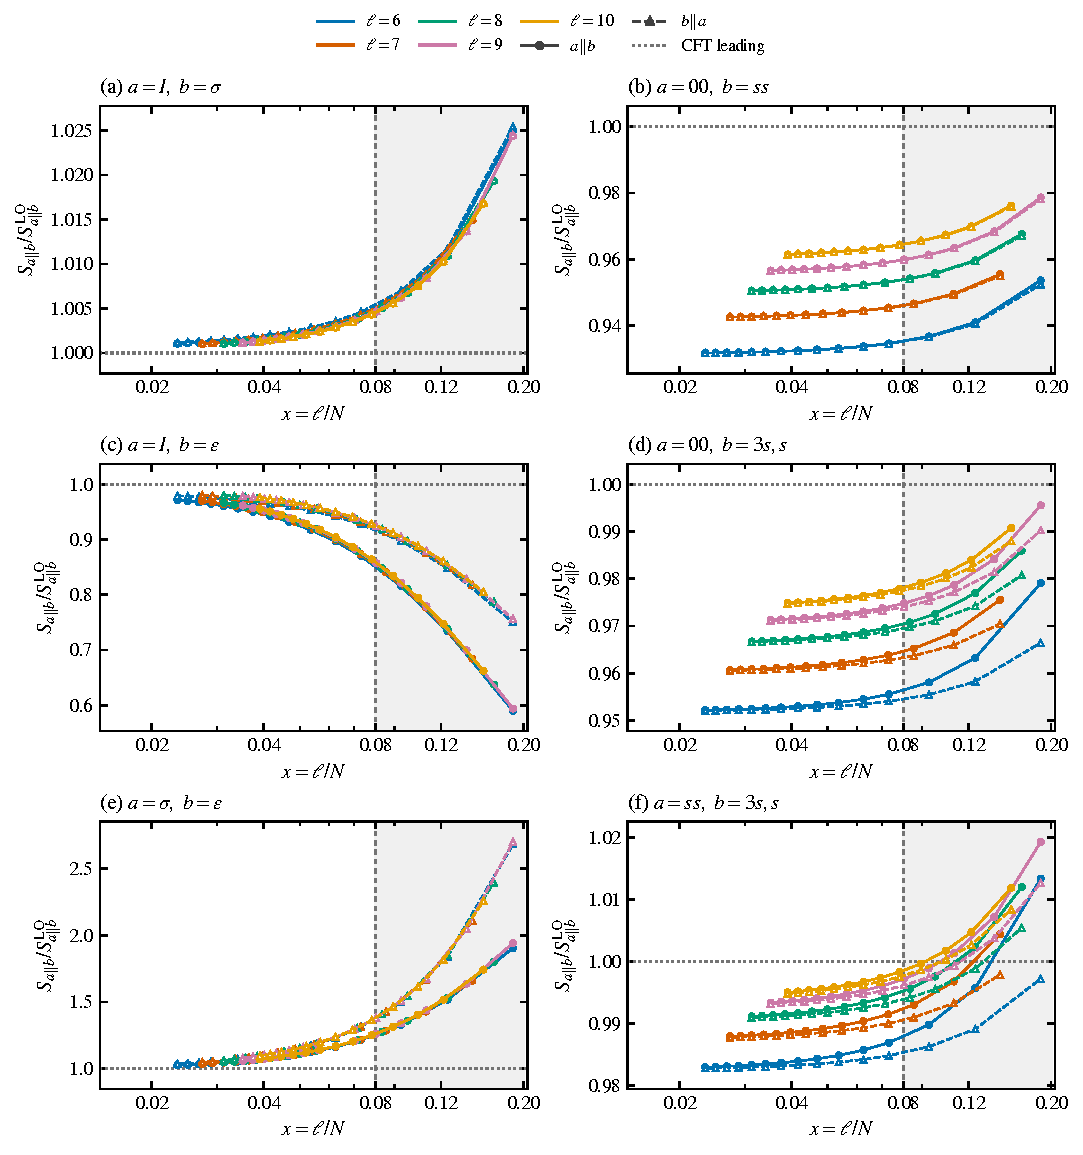
\includegraphics[width=.95\linewidth]{../figs/primary_entropy_leading.pdf}
\caption{Historical parameter-free leading-order check of primary relative entropy.
Each panel compares the two directions between the states $a,b$ named
in its title; the left column is Ising and the right column the compact
boson. The ordinate is $R=S_{a\Vert b}/[B_{ab}x^\alpha]$,
defined by Eq.~\eqref{eq:primary-comparison-metrics}; the dotted line
at one is the analytical CFT leading-order prediction. Colors identify
$\ell=6,\ldots,10$. Solid lines with filled circles denote $a\Vert b$,
and dashed lines with open triangles denote $b\Vert a$; segments only
connect computed sizes. Each direction has 70 points from the 15 sizes
through $N=256$ in Eq.~\eqref{eq:large-grid}, displayed for
$x\leq0.20$. The vertical line at $x=0.08$ marks the 51-point summary
window; shaded points are outside that window. There are no fitted
curves or optimized parameters. Ising uses exact Jordan--Wigner
primaries of $H=-\sum XX-\sum Z$ with periodic spins; the boson uses
the charges and $q=2$, $W=10^8$ construction in
Table~\ref{tab:boson-primary-entropy}. All logarithms are natural,
and the audited target-logarithm floor is $10^{-15}$.
$\alpha=4$, $B=8\pi^4/15$ for Ising $I\leftrightarrow\eps$;
$\alpha=2$, $B=\pi^2/12$ for the other Ising panels;
$\alpha=2$, $B=\pi^2/3,5\pi^2/3,2\pi^2/3$ for the boson panels from top to bottom.
Differences between reverse directions and departures from one remain
visible; the analytical equality is a leading-order statement.}
\label{fig:primary-entropy-leading}
\end{figure}
\clearpage
\subsection{Free power-law fits for the primary pairs}
\label{sec:primary-fits}
To test whether the numerical primary relative entropies recover both
parts of the analytical leading term, we fit one power law with a
free coefficient and a free exponent. The six-panel presentation follows
Figs.~\ref{fig:isingfits}--\ref{fig:bosonresid}; the fitting model below
is specific to the primary-pair comparison. The parameter-free checks
in Secs.~\ref{sec:primary-analytic}--\ref{sec:primary-results} remain
independent of these fits.

For a fixed directed pair $a\Vert b$, let $y_i=S_{a\Vert b}(x_i)$
denote a numerical observation. Define the fitted model and the
analytical leading prediction by
\begin{align}
 F(x;C,\alpha)&=Cx^\alpha,\qquad
 F_{\rm CFT}(x)=B_{ab}x^{\alpha_{\rm CFT}}, \notag\\
 (\widehat C,\widehat\alpha)
 &=\mathop{\mathrm{arg\,min}}_{C>0,\ \alpha\in\mathbb R}
   \sum_{i:x_i\leq0.08}\bigl[y_i-Cx_i^\alpha\bigr]^2 .
 \label{eq:primary-fit-ansatz}
\end{align}
Both $C$ and $\alpha$ are optimized, giving two free parameters.
No theoretical exponent or coefficient is supplied to the optimizer,
and the exponent is not restricted to an integer or to a neighborhood
of its CFT value. Positivity of $C$ enforces a positive power-law
entropy. This is unweighted nonlinear least squares in the entropy
itself; the logarithmic axes do not change the objective.
The analytical values $B_{ab}$ and $\alpha_{\rm CFT}$ from
Sec.~\ref{sec:primary-analytic} are used only for the subsequent
comparison. The CFT prediction has zero free parameters.

For a reproducible numerical procedure, set $x_\star=0.08$ and write
\begin{equation}
 t_i=\ln(x_i/x_\star),\quad
 F(x_i)=\exp(u+\alpha t_i),\quad
 C=\exp(u)x_\star^{-\alpha}.
 \label{eq:primary-free-pivot}
\end{equation}
First regress $\ln y_i$ on $t_i$ to obtain a data-based starting
guess for $(u,\alpha)$. Then optimize both variables against the
original entropies using Eq.~\eqref{eq:primary-fit-ansatz}.
The log-data regression supplies only an initial guess.
The solver uses derivatives
$\partial_uF=F$ and $\partial_\alpha F=Ft_i$;
rescaling all residuals by their common entropy scale does not
change the minimum. Finally convert the fitted amplitude to
$\widehat C$ using Eq.~\eqref{eq:primary-free-pivot}.

The fit uses 51 observations per direction from 12 contributing
system sizes, with the selection $\ell=6,\ldots,10$ and $x\leq0.08$.
The figures show 70 observations per direction from all 15 sizes
in Eq.~\eqref{eq:large-grid}, with $\ell=6,\ldots,10$ and $x\leq0.20$.
The 19 displayed observations outside $x\leq0.08$ do not affect any
coefficient or table metric. Curves beyond the vertical cutoff are
extrapolations of the fitted power law.

For clarity, define the signed entropy residual $r_i$, its percentage
$\eta_i$, and the root mean square error (RMSE), for either
$M=F$ or $M=F_{\rm CFT}$, by
\begin{equation}
 r_i=y_i-M(x_i),\qquad
 \eta_i=100\,\frac{r_i}{y_i},\qquad
 {\rm RMSE}_M=\sqrt{\frac{1}{51}\sum_{i:x_i\leq0.08}r_i^2}.
 \label{eq:primary-fit-residual}
\end{equation}
The percentage denominator here is the numerical entropy $y_i$.
It differs from the analytical denominator in
Eq.~\eqref{eq:primary-comparison-metrics}.
The two signed parameter deviations are
\begin{equation}
 \delta C[\%]=100\left(\frac{\widehat C}{B_{ab}}-1\right),
 \qquad
 \delta\alpha[\%]=100\left(
       \frac{\widehat\alpha}{\alpha_{\rm CFT}}-1\right).
 \label{eq:primary-parameter-errors}
\end{equation}
The coefficient comparison uses powers of $x$ itself, including all powers of $\pi$.
The archived amplitude $\widetilde C$ multiplying $(\pi x)^\alpha$
is converted by $C=\pi^\alpha\widetilde C$.
Changing this convention changes coefficient comparisons when the
exponents differ, so the convention must accompany the numbers.

Cross-validation (CV) omits one of the 12 contributing sizes,
refits \emph{both} parameters on the other 11, and predicts all
omitted observations. If $F^{(-N_i)}$ is the resulting prediction
for observation $i$, define
\begin{equation}
 {\rm CVRMSE}=\sqrt{\frac1{51}\sum_{i:x_i\leq0.08}
       [y_i-F^{(-N_i)}(x_i)]^2}.
 \label{eq:primary-free-cv}
\end{equation}
The residual degrees of freedom are $51-2=49$ for the free fit
and 51 for the analytical CFT leading-order prediction.
For the latter, CV RMSE equals RMSE because no parameter is refitted.

Tables~\ref{tab:ising-primary-all-fits}--\ref{tab:boson-primary-all-fits}
compare both fitted parameters with their analytical values.
For Ising, in the ordered-pair order of Table~\ref{tab:ising-primary-all-fits}, the fitted exponents are $2.0040, 2.0041, 3.8376, 3.9196, 2.2160, 2.3071$.
The boson exponents lie between $2.0050$ and $2.0090$.
The Ising spin--energy coefficients are $1.75660, 2.40358$, compared with $B_{ab}=\pi^2/12$.
A two-parameter power law over a finite window estimates an effective
coefficient and exponent; agreement of its curve with the data
does not by itself establish their asymptotic CFT values.
No additional term or lattice-correction model enters this fit.

\subsubsection{Complete Ising fitting table}
\label{sec:primary-ising-fit-table}
{\footnotesize\setlength{\tabcolsep}{3pt}\renewcommand{\arraystretch}{1.15}
\begin{longtable}{lrrrrrrrrr}
\caption{Ising primary-pair free power-law fits, $F(x)=\widehat Cx^{\widehat\alpha}$: both $C$ and $\alpha$ are optimized on 51 samples per direction, with $\ell=6,\ldots,10$, at $x\leq0.08$. The analytical CFT leading-order prediction is $B_{ab}x^{\alpha_{\rm CFT}}$, with no fitted parameters. All amplitudes include their powers of $\pi$. Parameter deviations use Eq.~\eqref{eq:primary-parameter-errors}; RMSE and CV RMSE refer to the free fit, and CFT RMSE to this analytical CFT prediction. Natural logarithms and the complete definitions in Sec.~\ref{sec:primary-fits} apply.}
\label{tab:ising-primary-all-fits}\\\toprule
Direction & $B_{ab}$ & $\widehat C$ & $\delta C$ [\%] & $\alpha_{\rm CFT}$ & $\widehat\alpha$ & $\delta\alpha$ [\%] & RMSE & CFT RMSE & CV RMSE\\\midrule\endfirsthead
\toprule
Direction & $B_{ab}$ & $\widehat C$ & $\delta C$ [\%] & $\alpha_{\rm CFT}$ & $\widehat\alpha$ & $\delta\alpha$ [\%] & RMSE & CFT RMSE & CV RMSE\\\midrule\endhead
\bottomrule\endfoot
$I\Vert \sigma$ & $1\pi^{2}/12$ & 0.8344 & 1.4505 & 2 & 2.004 & 0.20221 & $6.54\!\times\!10^{-7}$ & $7.21\!\times\!10^{-6}$ & $7.06\!\times\!10^{-7}$\\
$\sigma\Vert I$ & $1\pi^{2}/12$ & 0.83465 & 1.4819 & 2 & 2.0041 & 0.20553 & $7.67\!\times\!10^{-7}$ & $7.50\!\times\!10^{-6}$ & $8.33\!\times\!10^{-7}$\\
$I\Vert \varepsilon$ & $8\pi^{4}/15$ & 29.732 & -42.77 & 4 & 3.8376 & -4.059 & $2.44\!\times\!10^{-6}$ & $7.02\!\times\!10^{-5}$ & $2.64\!\times\!10^{-6}$\\
$\varepsilon\Vert I$ & $8\pi^{4}/15$ & 39.286 & -24.38 & 4 & 3.9196 & -2.01 & $1.95\!\times\!10^{-6}$ & $3.76\!\times\!10^{-5}$ & $2.23\!\times\!10^{-6}$\\
$\sigma\Vert \varepsilon$ & $1\pi^{2}/12$ & 1.7566 & 113.58 & 2 & 2.216 & 10.802 & $2.40\!\times\!10^{-5}$ & $3.95\!\times\!10^{-4}$ & $2.76\!\times\!10^{-5}$\\
$\varepsilon\Vert \sigma$ & $1\pi^{2}/12$ & 2.4036 & 192.24 & 2 & 2.3071 & 15.353 & $3.60\!\times\!10^{-5}$ & $5.66\!\times\!10^{-4}$ & $4.10\!\times\!10^{-5}$\\
\end{longtable}

}

\subsubsection{Complete compact-boson fitting table}
\label{sec:primary-boson-fit-table}
{\footnotesize\setlength{\tabcolsep}{3pt}\renewcommand{\arraystretch}{1.15}
\begin{longtable}{lrrrrrrrrr}
\caption{Compact-boson primary-pair free power-law fits, $F(x)=\widehat Cx^{\widehat\alpha}$: both $C$ and $\alpha$ are optimized on 51 samples per direction, with $\ell=6,\ldots,10$, at $x\leq0.08$. The analytical CFT leading-order prediction is $B_{ab}x^{\alpha_{\rm CFT}}$, with no fitted parameters. All amplitudes include their powers of $\pi$. Parameter deviations use Eq.~\eqref{eq:primary-parameter-errors}; RMSE and CV RMSE refer to the free fit, and CFT RMSE to this analytical CFT prediction. Natural logarithms and the complete definitions in Sec.~\ref{sec:primary-fits} apply.}
\label{tab:boson-primary-all-fits}\\\toprule
Direction & $B_{ab}$ & $\widehat C$ & $\delta C$ [\%] & $\alpha_{\rm CFT}$ & $\widehat\alpha$ & $\delta\alpha$ [\%] & RMSE & CFT RMSE & CV RMSE\\\midrule\endfirsthead
\toprule
Direction & $B_{ab}$ & $\widehat C$ & $\delta C$ [\%] & $\alpha_{\rm CFT}$ & $\widehat\alpha$ & $\delta\alpha$ [\%] & RMSE & CFT RMSE & CV RMSE\\\midrule\endhead
\bottomrule\endfoot
$00\Vert ss$ & $1\pi^{2}/3$ & 3.2114 & -2.3851 & 2 & 2.009 & 0.44964 & $9.35\!\times\!10^{-5}$ & $4.46\!\times\!10^{-4}$ & $1.07\!\times\!10^{-4}$\\
$ss\Vert 00$ & $1\pi^{2}/3$ & 3.2106 & -2.4094 & 2 & 2.0089 & 0.44594 & $9.36\!\times\!10^{-5}$ & $4.47\!\times\!10^{-4}$ & $1.07\!\times\!10^{-4}$\\
$00\Vert 3s,s$ & $5\pi^{2}/3$ & 16.286 & -0.99214 & 2 & 2.0079 & 0.39731 & $3.50\!\times\!10^{-4}$ & 0.0014811 & $4.02\!\times\!10^{-4}$\\
$3s,s\Vert 00$ & $5\pi^{2}/3$ & 16.231 & -1.3301 & 2 & 2.007 & 0.34759 & $3.62\!\times\!10^{-4}$ & 0.0015101 & $4.16\!\times\!10^{-4}$\\
$ss\Vert 3s,s$ & $2\pi^{2}/3$ & 6.6504 & 1.0737 & 2 & 2.0063 & 0.31743 & $7.02\!\times\!10^{-5}$ & $1.49\!\times\!10^{-4}$ & $8.04\!\times\!10^{-5}$\\
$3s,s\Vert ss$ & $2\pi^{2}/3$ & 6.6204 & 0.61876 & 2 & 2.005 & 0.25236 & $7.70\!\times\!10^{-5}$ & $1.65\!\times\!10^{-4}$ & $8.85\!\times\!10^{-5}$\\
\end{longtable}

}

\clearpage
\subsubsection{Reproducing the primary fits}
The command module \path{src/conformal_blocks/primary_fits.py} calls
\path{primary_powerlaw.py} on the existing direct measurements
in \path{primary_relative_entropy.csv}; no density matrix is recomputed.
Its separate outputs in \path{report/data/} are
\path{primary_fit_summary.csv} (24 free/CFT summaries),
\path{primary_fit_input.csv} (612 selected observations),
\path{primary_fit_residuals.csv} (1224 selected residuals),
\path{primary_display_input.csv} (840 displayed observations),
\path{primary_display_predictions.csv} (1680 displayed predictions),
\path{primary_exact_coefficients.csv} (12 analytical leading terms),
and \path{primary_free_power_cv.csv} (144 omitted-size refits).
The public entropy column is \path{S_primary}.
The full summary CSV retains both parameter estimates and deviations,
squared-error sums, relative-residual indicators from Eq.~\eqref{eq:metrics},
and the minimum and maximum of both parameters across the 12 CV fits.
Its additional local diagnostics use the Jacobian
$J_{i1}=F_i$, $J_{i2}=F_it_i$ in variables $(u,\alpha)$:
$\kappa_J=\sigma_{\max}(J)/\sigma_{\min}(J)$ and the covariance
$({\rm SSE}/49)(J^TJ)^{-1}$. Transforming this covariance to
$(C,\alpha)$ gives a matrix $V$. The exported standard errors are
$\sqrt{V_{11}}$ and $\sqrt{V_{22}}$, and the parameter correlation
is $V_{12}/\sqrt{V_{11}V_{22}}$.
These local linearization diagnostics are descriptive, not confidence
intervals for correlated lattice data.

The archived solver CSV uses its original $(\pi x)^\alpha$ amplitude.
The report converter writes \path{primary_reported_coefficients.csv}
with $C=\pi^{\widehat\alpha}\widetilde C$ and
$B_{ab}=\pi^{\alpha_{\rm CFT}}\widetilde B_{ab}$, including the
transformed coefficient errors and local covariance. Physical curves,
exponents and residuals are invariant under this conversion.

An independent check eliminates the amplitude at each trial exponent:
\begin{equation}
 \widehat A(\alpha)=
  \frac{\sum_i y_i v_i(\alpha)}{\sum_i v_i(\alpha)^2},
 \qquad v_i(\alpha)=(x_i/x_\star)^\alpha .
 \label{eq:primary-profile-check}
\end{equation}
Minimizing the remaining one-dimensional objective independently checks
the two-parameter solver. This check covers all 12 complete fits
and all 144 omitted-size fits; a synthetic power law with the
noninteger exponent $2.37$ also verifies that the solver recovers
a free exponent. The implementation is
\path{report/primary_free_fit_checks.py}.
With the interpreter variable \path{PY} defined in
Sec.~\ref{sec:primary-results}, run from the project root:
\begin{verbatim}
PYTHONPATH=src $PY -m conformal_blocks.primary_fits
PYTHONPATH=src MPLCONFIGDIR=/tmp/relative_entropy_mpl \
  $PY report/primary_fit_artifacts.py
PYTHONPATH=src $PY report/primary_free_fit_checks.py
\end{verbatim}
The renderer reads these CSVs to generate the four vector PDF figures
and Tables~\ref{tab:ising-primary-all-fits}--\ref{tab:boson-primary-all-fits}.

\clearpage
\begin{figure}[p]\centering
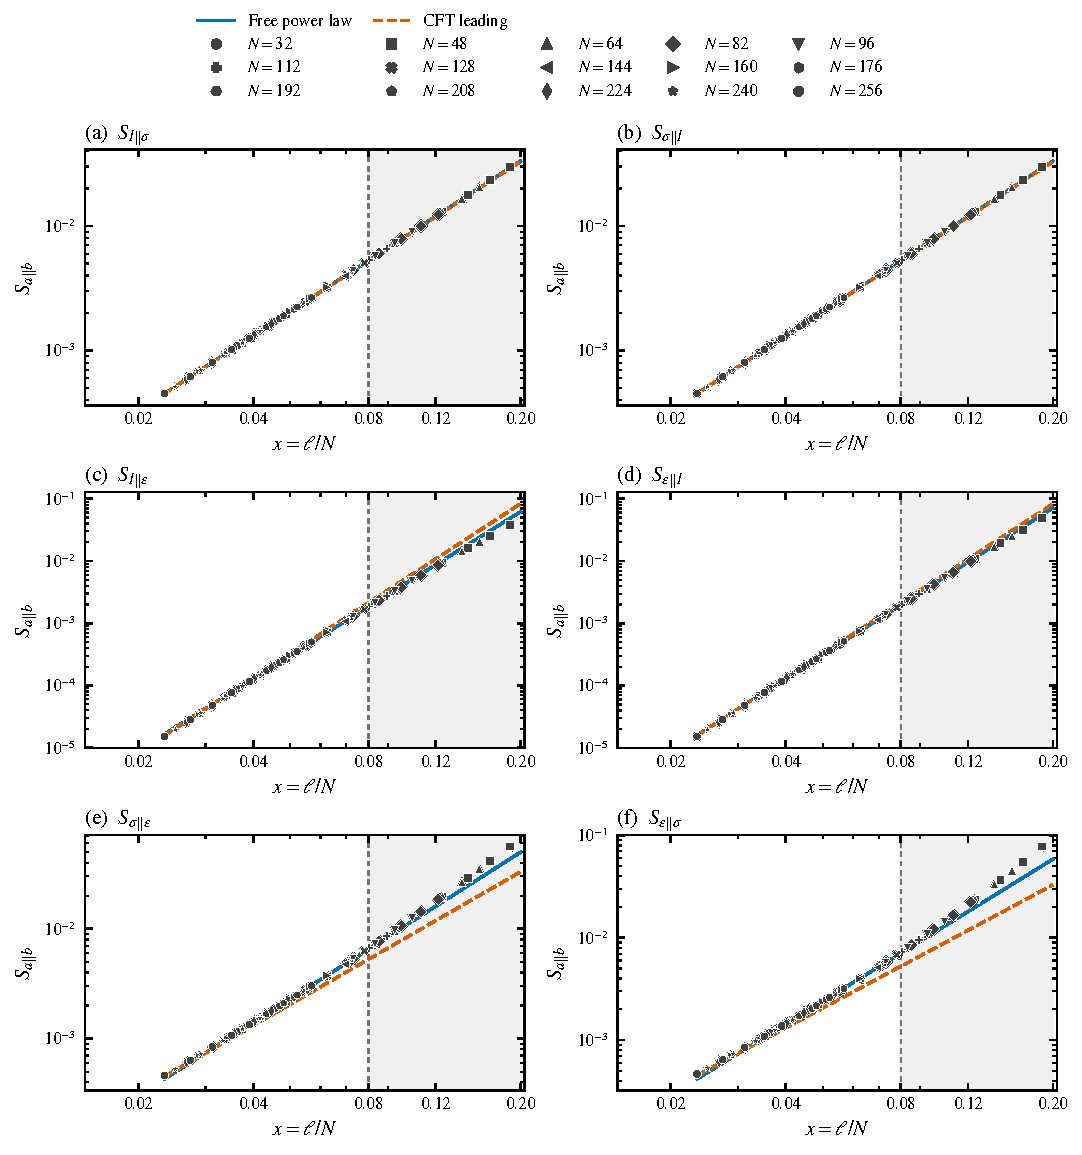
\includegraphics[width=.95\linewidth]{../figs/ising_primary_fits.pdf}
\caption{Historical Ising primary relative entropy $S_{a\Vert b}$ for
all six directions. Markers identify the 15 system sizes through
$N=256$ in Eq.~\eqref{eq:large-grid}; $\ell=6,\ldots,10$.
Each panel shows 70 observations with $x=\ell/N\leq0.20$.
Only the 51 observations at $x\leq0.08$ enter the unweighted
least-squares fits in Eq.~\eqref{eq:primary-fit-ansatz}.
The vertical line and shading mark the cutoff and the extrapolation
region containing 19 observations. Blue solid lines show the free
power law $F=\widehat Cx^{\widehat\alpha}$; both parameters
are optimized independently for each direction. Orange dashed
lines show the analytical CFT leading-order prediction, with no fitted parameters. For panels (c,d),
$\alpha_{\rm CFT}=4$ and $B_{ab}=8\pi^4/15$; elsewhere
$\alpha_{\rm CFT}=2$ and $B_{ab}=\pi^2/12$.
Table~\ref{tab:ising-primary-all-fits} compares both fitted
parameters with these analytical values.
The data use exact Jordan--Wigner primaries of the critical
periodic-spin Hamiltonian $H=-\sum XX-\sum Z$,
natural logarithms, and target-logarithm floor $10^{-15}$.
Both axes are logarithmic. The fitted exponent is a free real
number and the coefficient is positive; no additional powers enter.}
\label{fig:ising-primary-fits}
\end{figure}

\begin{figure}[p]\centering
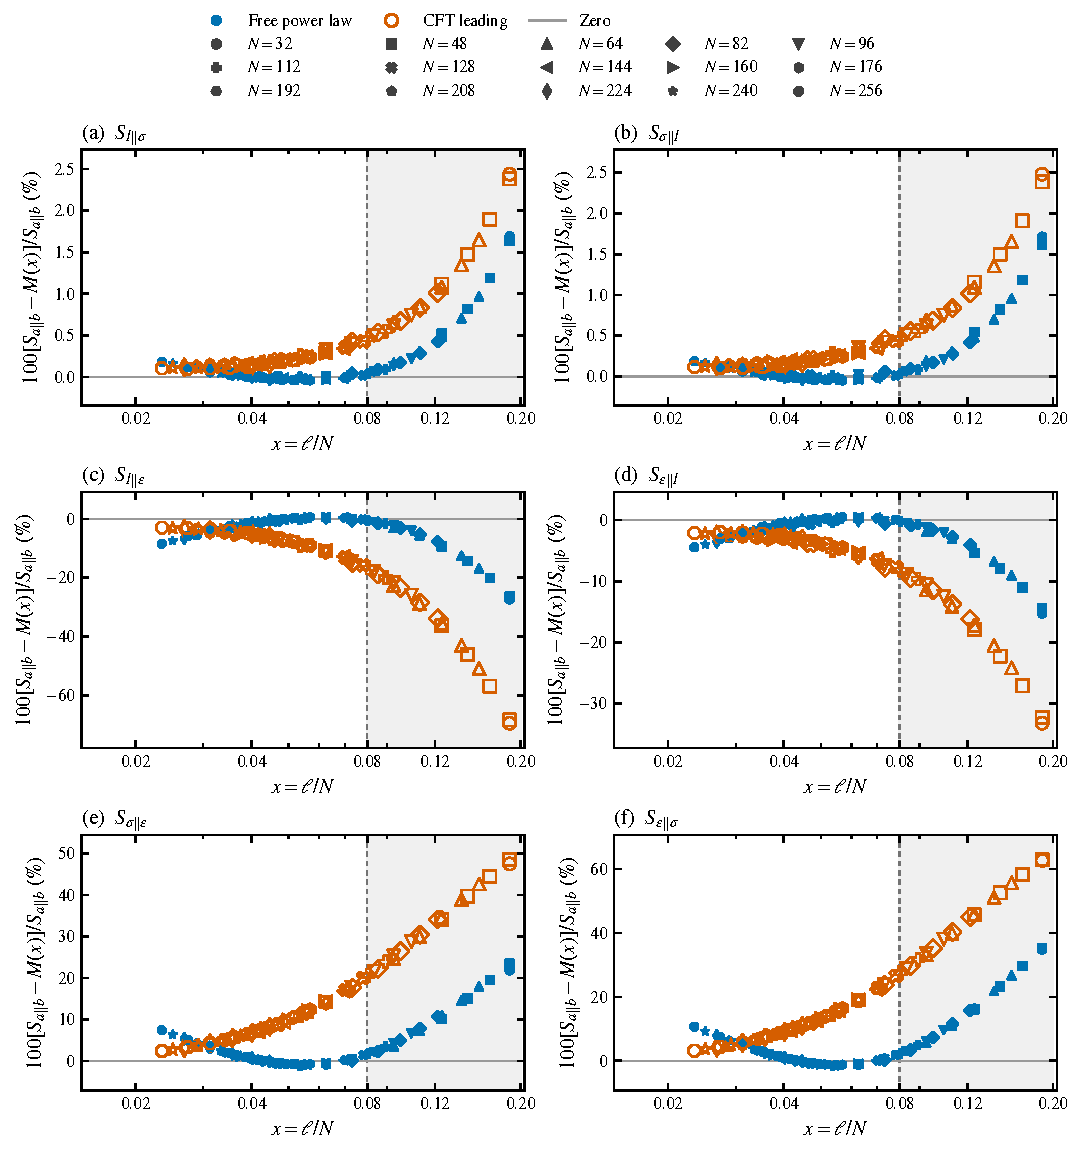
\includegraphics[width=.95\linewidth]{../figs/ising_primary_residuals.pdf}
\caption{Signed percentage residuals for the Ising primary
comparisons in Fig.~\ref{fig:ising-primary-fits}. Blue filled markers
denote the free power law and orange open markers the analytical
leading prediction. Marker shapes identify the 15 sizes in
Eq.~\eqref{eq:large-grid}, with
$\ell=6,\ldots,10$. The ordinate is
$\eta_i=100[S_{a\Vert b}(x_i)-M(x_i)]/S_{a\Vert b}(x_i)$,
where $M=F$ or $F_{\rm CFT}$,
from Eq.~\eqref{eq:primary-fit-residual}; zero means exact agreement.
The ordinate is linear throughout, with ticks showing signed percentage
values directly; $x$ is logarithmic.
All 70 displayed observations per direction satisfy $x\leq0.20$.
Only 51 at $x\leq0.08$ determine the fits and table metrics;
the 19 shaded-region observations test extrapolation.
The free fit has two jointly optimized parameters,
$F=\widehat Cx^{\widehat\alpha}$.
Only the analytical comparison uses $\alpha_{\rm CFT}=4$,
$B_{ab}=8\pi^4/15$ in (c,d), and $\alpha_{\rm CFT}=2$, $B_{ab}=\pi^2/12$
otherwise. The exact PBC Ising states, natural
logarithms and target floor $10^{-15}$ are as in
Fig.~\ref{fig:ising-primary-fits}; coefficients, exponents, RMSE and
CV RMSE appear in Table~\ref{tab:ising-primary-all-fits}.}
\label{fig:ising-primary-residuals}
\end{figure}

\begin{figure}[p]\centering
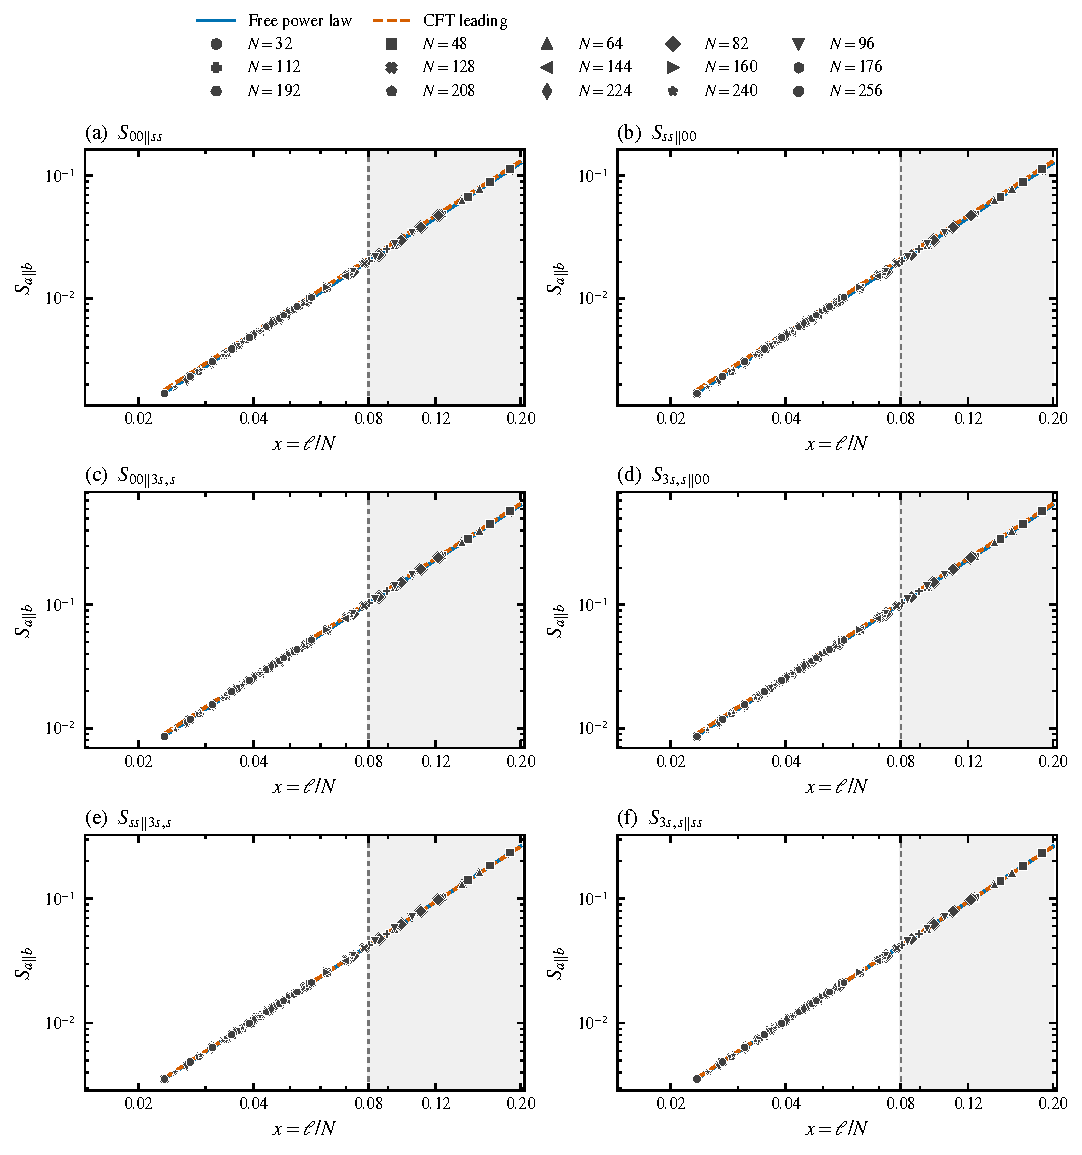
\includegraphics[width=.95\linewidth]{../figs/boson_primary_fits.pdf}
\caption{Historical compact-boson primary relative entropy for all six
directions among charges $(0,0)$, $(s,s)$ and $(3s,s)$,
$s=1/\sqrt2$. Markers identify the 15 sizes through $N=256$
in Eq.~\eqref{eq:large-grid}; $\ell=6,\ldots,10$.
Each panel displays 70 observations at $x\leq0.20$.
The 51 observations at $x\leq0.08$ determine the unweighted
least-squares fits; the vertical line and shading mark the 19
observations outside the fit window. Blue solid lines show
$F=\widehat Cx^{\widehat\alpha}$ from
Eq.~\eqref{eq:primary-fit-ansatz}, with both coefficient and exponent
optimized. Orange dashed lines show the analytical CFT leading-order
predictions, with no fitted parameters: $\alpha_{\rm CFT}=2$ and
$B_{ab}=\pi^2/3$ in (a,b), $5\pi^2/3$ in (c,d), and $2\pi^2/3$ in (e,f).
Table~\ref{tab:boson-primary-all-fits} compares both fitted
parameters with the analytical values.
The normalized vertex/Jastrow states use the unit circle,
$q=2$, $w_1=0$, $W=10^8$, and 100-decimal-digit Pfaffian
construction, without orthogonalization, as in
Sec.~\ref{sec:primary-numerics}.
All logarithms are natural and the target-logarithm floor
is $10^{-15}$. Both axes are logarithmic. The fit has a positive
coefficient and a free real exponent, with no additional terms.}
\label{fig:boson-primary-fits}
\end{figure}

\begin{figure}[p]\centering
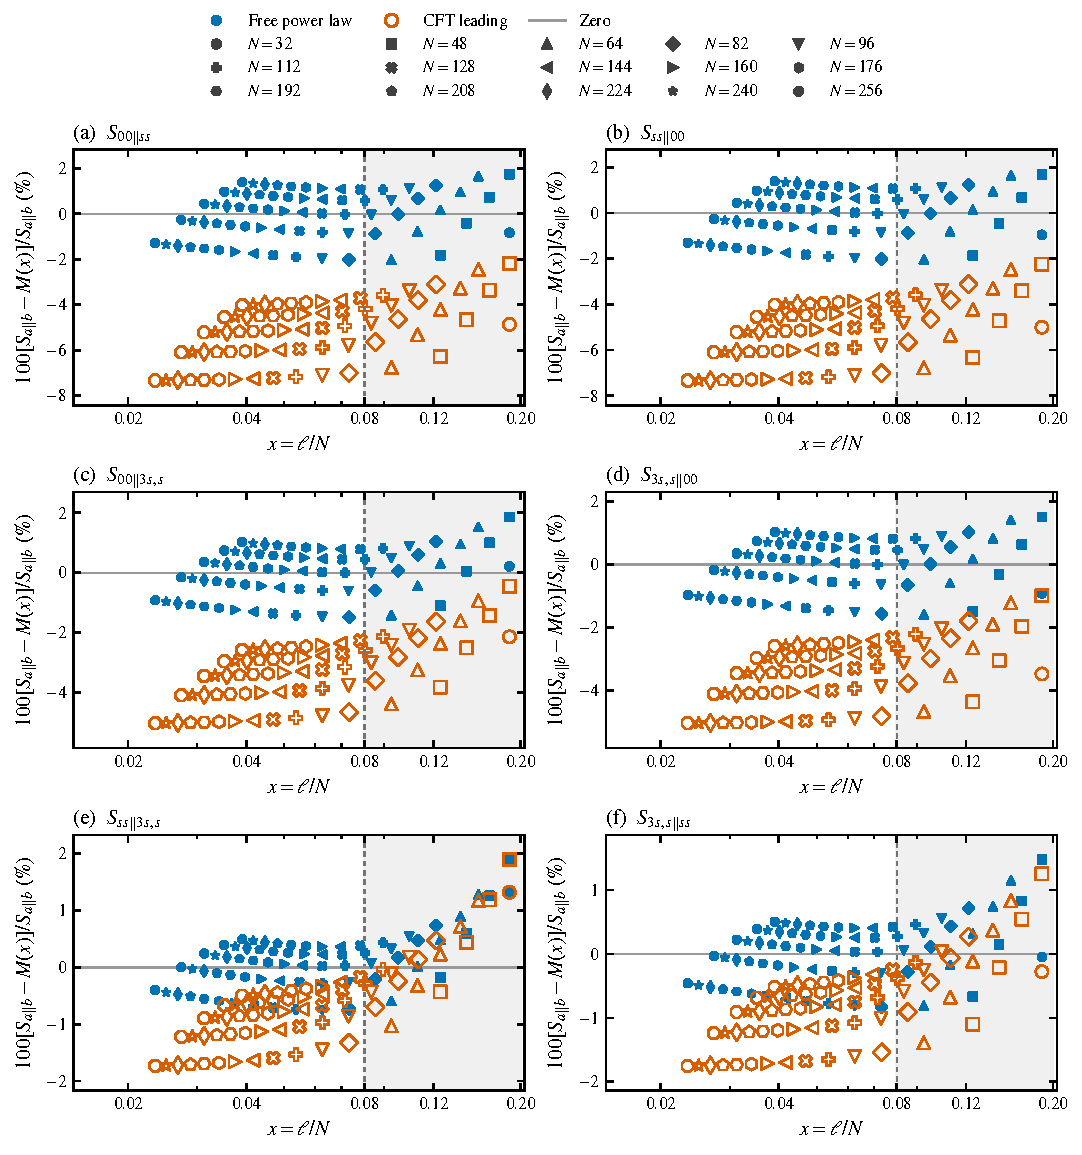
\includegraphics[width=.95\linewidth]{../figs/boson_primary_residuals.pdf}
\caption{Signed percentage residuals for the compact-boson
primary comparisons in Fig.~\ref{fig:boson-primary-fits}.
Blue filled markers denote the free power law; orange open markers
denote the analytical leading term.
The ordinate is $100[S_{a\Vert b}-M]/S_{a\Vert b}$,
where $M=F$ or $F_{\rm CFT}$,
as in Eq.~\eqref{eq:primary-fit-residual}. The vertical scale is linear
throughout, with ticks showing signed percentage values directly;
$x$ is logarithmic. Markers identify the 15 sizes in
Eq.~\eqref{eq:large-grid}, with $\ell=6,\ldots,10$.
All 70 observations per direction at $x\leq0.20$ are shown;
51 at $x\leq0.08$ enter the fits and metrics, while 19 lie
in the shaded extrapolation region. The two-parameter fit is
$F=\widehat Cx^{\widehat\alpha}$; its exponent is not
fixed. The analytical comparison uses $\alpha_{\rm CFT}=2$
and $B_{ab}=\pi^2/3$, $5\pi^2/3$, $2\pi^2/3$ in the top, middle and bottom rows.
The vertex charges, $q=2$,
unit-circle sites, $w_1=0$, $W=10^8$, 100-digit construction,
absence of orthogonalization, natural logarithms and
target floor $10^{-15}$ are as in Fig.~\ref{fig:boson-primary-fits}.
Table~\ref{tab:boson-primary-all-fits} compares fitted coefficients
and exponents with theory and gives RMSE and size-based CV RMSE.}
\label{fig:boson-primary-residuals}
\end{figure}
\clearpage

